% ResumeLens research poster — fully editable LaTeX source
% Page: A2 landscape, 594 x 420 mm
% Compile: xelatex -interaction=nonstopmode ResumeLens_Research_Poster.tex
\documentclass{article}
\usepackage[a2paper,landscape,margin=0mm]{geometry}
\usepackage{iftex}
\ifxetex
  \usepackage{fontspec}
  \setmainfont{Arial}
  \setsansfont{Arial}
  \setmonofont{Consolas}[Scale=0.88]
\else
  \usepackage[T1]{fontenc}
  \usepackage[utf8]{inputenc}
  \usepackage{helvet}
  \renewcommand{\familydefault}{\sfdefault}
  \usepackage{inconsolata}
\fi
\usepackage{tikz}
\usetikzlibrary{calc,positioning,arrows.meta}
\usepackage{amsmath,amssymb,booktabs,array}
\usepackage{ragged2e}
\pagestyle{empty}
\setlength{\parindent}{0pt}
\setlength{\parskip}{0pt}
\definecolor{navy}{HTML}{15355B}
\definecolor{blue}{HTML}{1671AC}
\definecolor{pale}{HTML}{ECF5FA}
\definecolor{ink}{HTML}{273D50}
\definecolor{green}{HTML}{16835F}
\definecolor{bg}{HTML}{F7FAFC}
\definecolor{line}{HTML}{C9DCEB}
\newcommand{\B}{\color{navy}\bfseries}
\newcommand{\bodyfont}{\fontsize{14.5}{19.1}\selectfont}
\newcommand{\subfont}{\fontsize{13.5}{17.6}\selectfont}
\newcommand{\codefont}{\fontsize{12}{16.7}\selectfont\ttfamily}
\newcommand{\panelsize}{18.0}
\newcommand{\panel}[5]{%
  % x [cm], y from top [cm], height [cm], heading, body
  \pgfmathsetmacro{\xend}{#1+\panelsize}
  \pgfmathsetmacro{\ytop}{42.0 - #2}
  \pgfmathsetmacro{\ybot}{42.0 - #2 - #3}
  \pgfmathsetmacro{\yhead}{42.0 - #2 - 0.50}
  \pgfmathsetmacro{\yline}{42.0 - #2 - 1.23}
  \pgfmathsetmacro{\ybody}{42.0 - #2 - 1.58}
  \pgfmathsetmacro{\xhead}{#1+0.48}
  \pgfmathsetmacro{\xlinestart}{#1+0.46}
  \pgfmathsetmacro{\xlineend}{#1+17.53}
  \pgfmathsetmacro{\xbody}{#1+0.49}
  \fill[white,rounded corners=4mm] (#1,\ytop) rectangle (\xend,\ybot);
  \draw[draw=line,rounded corners=4mm,line width=0.6pt] (#1,\ytop) rectangle (\xend,\ybot);
  \node[anchor=north west,inner sep=0,text width=17.0cm,font=\bfseries\fontsize{19}{23}\selectfont,text=navy] at (\xhead,\yhead) {#4};
  \draw[blue,line width=1.2pt] (\xlinestart,\yline) -- (\xlineend,\yline);
  \node[anchor=north west,inner sep=0,align=left,text width=17.0cm,font=\bodyfont,text=ink] at (\xbody,\ybody) {#5};
}
\begin{document}%
\noindent\begin{tikzpicture}[x=1cm, y=1cm]
\useasboundingbox (0,0) rectangle (59.4, 42.0);
% Background, masthead and footer
\fill[bg] (0,0) rectangle (59.4, 42.0);
\fill[navy] (0, 36.85) rectangle (59.4, 42.0);
\fill[blue] (0, 36.68) rectangle (59.4, 36.85);
\node[anchor=north,align=center,text=white,font=\bfseries\fontsize{51}{59}\selectfont] at (29.7, 41.38) {ResumeLens};
\node[anchor=north,align=center,text=white,font=\fontsize{24}{30}\selectfont] at (29.7, 39.75) {Formal-Language Models for Transparent R\'esum\'e Screening};
\node[anchor=north,align=center,text=white!88,font=\fontsize{15}{20}\selectfont] at (29.7, 38.45) {Johan Mora \quad\textbullet\quad Joshua Sayur \quad\textbullet\quad Juan David Fajardo};
\node[anchor=north,align=center,text=white!88,font=\fontsize{14}{18}\selectfont] at (29.7, 37.75) {Universidad Icesi \quad | \quad Computaci\'on y Estructuras Discretas III \quad | \quad 2026-2};

% --- Left column ---
\panel{1.7}{6.0}{8.9}{01 \quad Problem and objective}{
R\'esum\'es express similar qualifications with different names, spellings, and abbreviations. Literal keyword matching can miss skills or treat equivalent expressions as unrelated.
\par\vspace{0.20cm}
{\B Research objective.} Extract explicit candidate evidence, normalize technical qualifications, recognize formal patterns for four job profiles, and validate a structured candidate specification.
\par\vspace{0.22cm}
\colorbox{pale}{\parbox{15.95cm}{\vspace{0.16cm}\textbf{Research question}\par\smallskip How can formal-language models make r\'esum\'e screening more interpretable, consistent, and auditable?\vspace{0.16cm}}}
\par\vspace{0.18cm}
{\subfont The tool does not rank people or make hiring decisions.}
}
\panel{1.7}{15.35}{12.0}{02 \quad End-to-end architecture}{
\centering
\begin{tikzpicture}[>=Latex,node distance=0.37cm,
 stage/.style={draw=blue!40,fill=pale,rounded corners=5pt,minimum height=1.33cm,text width=14.9cm,align=center,font=\fontsize{14}{17}\selectfont}]
 \node[stage] (r) {\textbf{1. Extract}\quad Python \texttt{re}};
 \node[stage,below=of r] (n) {\textbf{2. Normalize}\quad finite-state transducers};
 \node[stage,below=of n] (d) {\textbf{3. Recognize}\quad four DFA classifiers};
 \node[stage,below=of d] (g) {\textbf{4. Validate}\quad EBNF + textX grammar};
 \node[stage,below=of g] (o) {\textbf{5. Render}\quad HTML / Markdown profile};
 \foreach \a/\b in {r/n,n/d,d/g,g/o}{\draw[->,very thick,blue] (\a) -- (\b);}
\end{tikzpicture}
\par\vspace{0.25cm}
\RaggedRight
{\subfont \texttt{run\_pipeline()} coordinates every stage. The same program evaluates all four supported profiles. Intermediate outputs remain inspectable.}
}
\panel{1.7}{27.8}{11.15}{03 \quad Regex extraction}{
Python regular expressions identify personal/contact information, education, professional experience, and technical qualifications. The extraction stage does \emph{not} classify a candidate.
\par\vspace{0.23cm}
{\B Example input}\par\smallskip
{\codefont Wednesday Addams\par Technical Skills: JS, React.js, NodeJS,\par Postgres, Git}
\par\vspace{0.22cm}
{\B Extracted qualification tokens}\par\smallskip
{\codefont [JS, React.js, NodeJS, Postgres, Git]}
\par\vspace{0.25cm}
{\subfont Regex identifies textual patterns; the following FST stage resolves equivalent technology names.}
}

% --- Center column ---
\panel{20.7}{6.0}{15.8}{04 \quad Normalization with FSTs}{
Nine genuine \texttt{pyformlang.fst.FST} instances normalize aliases by technological family. Each is described by the formal seven-tuple:
\[\textstyle T=(Q,\Sigma,\Gamma,\delta,\omega,q_0,F)\]
Inputs are read character by character. Intermediate transitions emit the empty output $\varepsilon$; a completed alias produces its canonical skill token.
\par\vspace{0.17cm}
{\B Examples of transformations}\par\vspace{0.10cm}
{\subfont
\begin{tabular}{@{}p{7.0cm}p{8.9cm}@{}}
\toprule
\textbf{Variant input} & \textbf{Canonical output}\\
\midrule
\texttt{JS} & \texttt{JAVASCRIPT}\\
\texttt{React.js} & \texttt{REACT}\\
\texttt{NodeJS} & \texttt{NODE\_JS}\\
\texttt{Postgres} & \texttt{POSTGRESQL}\\
\texttt{sklearn} & \texttt{SCIKIT\_LEARN}\\
\texttt{Tensor Flow} & \texttt{TENSORFLOW}\\
\bottomrule
\end{tabular}}
\par\vspace{0.28cm}
{\color{green}\bfseries 9 FSTs} \quad\textbullet\quad 35 canonical technologies\\
{\subfont Aliases are grouped by families, rather than building one transducer per input word.}
}
\panel{20.7}{22.25}{16.7}{05 \quad Recognition with four DFAs}{
Each profile is recognized by a deterministic finite automaton:
\[\textstyle A=(Q,\Sigma,\delta,q_0,F)\]
States encode subsets of satisfied mandatory categories. With $k$ required categories, the shared construction creates $2^k$ states. Optional skills induce self-loops; skill order does not determine acceptance.
\par\vspace{0.25cm}
{\subfont
\begin{tabular}{@{}p{12.6cm}r@{}}
\toprule
\textbf{Profile} & \textbf{States}\\
\midrule
Full Stack Developer & 32\\
Machine Learning Engineer & 64\\
QA Engineer & 64\\
Data Analyst & 16\\
\bottomrule
\end{tabular}}
\par\vspace{0.17cm}
{\B Conceptual cumulative recognition}
\begin{center}
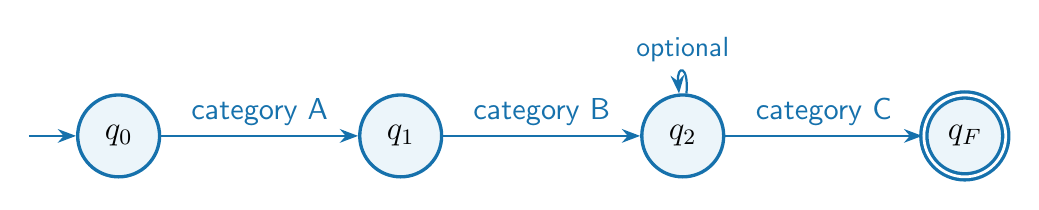
\begin{tikzpicture}[>=Stealth,node distance=2.50cm,
st/.style={circle,fill=pale,draw=blue,very thick,minimum size=1.04cm,font=\fontsize{12}{14}\selectfont}]
\node[st] (q0) {$q_0$};
\node[st,right=of q0] (q1) {$q_1$};
\node[st,right=of q1] (q2) {$q_2$};
\node[st,right=of q2,double,double distance=1pt] (qf) {$q_F$};
\draw[->,blue,thick] ($(q0.west)+(-0.6,0)$) -- (q0.west);
\draw[->,blue,thick] (q0) -- node[above,font=\fontsize{11}{13}\selectfont] {category A} (q1);
\draw[->,blue,thick] (q1) -- node[above,font=\fontsize{11}{13}\selectfont] {category B} (q2);
\draw[->,blue,thick] (q2) -- node[above,font=\fontsize{11}{13}\selectfont] {category C} (qf);
\draw[->,blue,thick] (q2) to[out=85,in=95,looseness=10] node[above,font=\fontsize{10}{12}\selectfont] {optional} (q2);
\end{tikzpicture}
\end{center}
{\subfont \textit{Schematic illustration only; the repository includes complete DOT transition diagrams for all four DFAs.}}
}

% --- Right column ---
\panel{39.7}{6.0}{13.5}{06 \quad Candidate DSL and textX}{
The DSL represents candidate details, education, experience, technical skills, and classification. A context-free grammar is formalized in EBNF and implemented using \texttt{resume.tx} and textX.
\par\vspace{0.24cm}
{\B Example candidate-language fragment}\par\vspace{0.15cm}
\colorbox{pale}{\parbox{15.9cm}{\vspace{0.15cm}\codefont
candidate "Wednesday Addams" \{\par
\hspace*{0.6cm}experience \{ years: 3 \}\par
\hspace*{0.6cm}skills \{ JAVASCRIPT, REACT,\par
\hspace*{1.50cm}NODE\_JS, POSTGRESQL, GIT \}\par
\hspace*{0.6cm}classification \{\par
\hspace*{1.25cm}FULL\_STACK\_DEVELOPER: ACCEPTED\par
\hspace*{0.6cm}\}\par
\}\vspace{0.15cm}}}
\par\vspace{0.24cm}
{\subfont \textbf{Two layers of validation:} lexical/syntactic grammar checks and semantic checks (nonempty names; 0--60 experience years; unique skills and unique profile results).}
}
\panel{39.7}{19.9}{11.8}{07 \quad Results and test evidence}{
\centering
{\color{green}\fontsize{50}{55}\selectfont\bfseries 345}\par\vspace{-0.1cm}
{\bfseries automated tests passed in the final local audit}
\par\vspace{0.33cm}
\RaggedRight
{\subfont
\begin{tabular}{@{}p{7.9cm}p{8.1cm}@{}}
\toprule
\textbf{Sample r\'esum\'e} & \textbf{Accepted profile}\\
\midrule
Wednesday Addams & Full Stack Developer\\
Mary Jane Watson & Machine Learning Engineer\\
QA example & QA Engineer\\
Data Analyst example & Data Analyst\\
\bottomrule
\end{tabular}}
\par\vspace{0.28cm}
{\subfont End-to-end CLI tests also covered empty input, unknown technologies, and invalid experience ranges. The latest audit did not independently verify browser interaction with the Streamlit UI.}
}
\panel{39.7}{32.1}{6.85}{08 \quad Limitations and conclusions}{
{\subfont \textbf{Limitations:} Results depend on explicit textual evidence; the tool cannot infer missing qualifications or assess overall hiring suitability.}
\par\vspace{0.18cm}
{\subfont \textbf{Conclusion:} Combining Regex, FSTs, DFAs and a CFG offers an interpretable, modular, testable qualification-pattern pipeline.}
\par\vspace{0.23cm}
{\fontsize{11.8}{15.5}\selectfont
\textbf{Selected references:} [1] Hopcroft, Motwani \& Ullman, \emph{Introduction to Automata Theory, Languages, and Computation} (2006). [2] Mohri, \emph{Finite-State Transducers in Language and Speech Processing} (1997). [3] textX documentation (textx.github.io).}
}
% Bottom small footer
\node[anchor=south,text=ink!68,font=\fontsize{12}{15}\selectfont] at (29.7, 0.6) {ResumeLens \; | \; Formal-language-based qualification recognition \; | \; Research poster for Integrative Task 1};
\end{tikzpicture}
\end{document}
